\documentclass[10pt]{report}
\usepackage{/Users/bradenhoagland/latex/math}

\lhead{Braden Hoagland}
\chead{Algebraic Structures II}
\rhead{}

\begin{document}

\begin{titlepage}
        \vspace*{\stretch{1.0}}
        \begin{center}
		{\Huge\textbf{Algebra (II)}}\\
                \vspace{4mm}
                Fields, Modules, and Galois Theory\\
                \vspace{6mm}
                \textit{Braden Hoagland}
        \end{center}
        \begin{figure}[H]
                \centering
                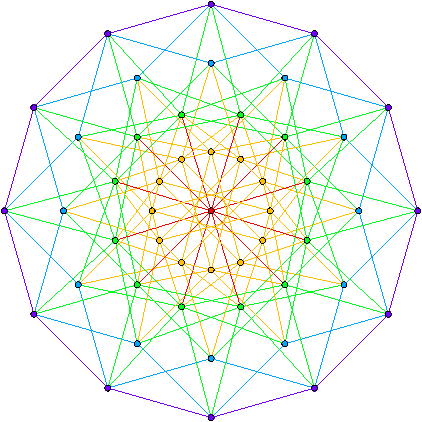
\includegraphics[scale=1]{fig/hey.pdf}
        \end{figure}
        \vspace*{\stretch{2.0}}

\end{titlepage}

\tableofcontents

\begin{defn}[]
	A field $K$ is a \textbf{(field) extension} of $F$ if $F$ is a subfield of $K$. Denote this by $K\nwarrow F$.
\end{defn}

\begin{defn}
	If $K$ is an extension of $F$, then the \textbf{degree} $[K:F]$ of $K$ over $F$ is the dimension of $K$ as an $F$-vector space. An extension is \textbf{finite} if its degree is finite, and its \textbf{infinite} otherwise.
\end{defn}

\begin{ex}[]
	$[\mathbb{C}:\mathbb{R}]=2$ because $\left\{ 1,i \right\}$ is a basis for $\mathbb{C}$ over $\mathbb{R}$.
\end{ex}

Many field extensions arise from trying to solve polynomial equations, so we gotta review that.

\begin{thrm}[]
	Let $F$ be a field, then $F[x]$ is a Euclidean Domain.
\end{thrm}

This means that any polynomial ring over a field has a division algorithm, i.e. for all $f(x)$ and nonzero $g(x)$, there exist \textit{unique} $q(x), r(x)$ such that
\[
	f(x)=q(x)g(x)+r(x),
\] where $\deg r(x) < \deg g(x)$. Here, we take the degree of the zero polynomial to be 0. It should also be clear that degree is the norm of $F[x]$.

\begin{cor}
	$F[x]$ is also a principal ideal domain (PID) and a unique factorization domain (UFD).
\end{cor}

If $E \nwarrow F$ and $f(x), 0 \neq g(x) \in F[x]$, then the result of the division algorithm in $F[x]$ is the same in $E[x]$ by the uniqueness bit. {\color{red}paragraph at end of sec 9.2.}

Often, even if $R$ is not a field (but \textit{is} a UFD), then we can say something about factorization in $R$ by looking at its field of fractions {\color{red}(the smallest field containing $R$, see sec 7.5, think $\mathbb{Z}$ to $\mathbb{Q}$).}

\begin{lem}[Gauss' Lemma]
	Let $R$ be a UFD with field of fractions $F$. Let $p(x) \in R[x]$ have coefficients with $\gcd$ 1, then $p(x)$ is irreducible in $R[x]$ if and only if it's irreducible in $F[x]$.
\end{lem}

Note that this works for all monic polynomials.

\begin{prop}
	Let $p(x) \in F[x]$, where $F$ is a field. Then $p(x)$ has a root $a \in F$ if and only if $(x-a)$ divides $p(x)$.
\end{prop}
\begin{proof}
	{\color{red}Do this.}
\end{proof}

\begin{cor}
	Any $p(x) \in F[x]$ has at most $\deg p$ roots in $F$ (including with multiplicity).
\end{cor}
\begin{proof}
	Use induction on the proposition above.
\end{proof}

\begin{cor}
	\label{cor:2-3-reducible}
	If $p(x) \in F[x]$ has degree 2 or 3, then it's reducible if and only if it has a root in $F$.
\end{cor}

The above corollary should be relatively obvious, but note that it doesn't hold in 4 dimensions or higher because a reducible polynomial could reduce into two other polynomials that have dimension 2+.

\begin{ex}[]
	We claim that $p(x) = x^3+x+1$ is irreducible in $\mathbb{F}_{2}[x]$. Using Corollary \ref{cor:2-3-reducible}, we check that $p(0)$ and $p(1)$ are nonzero, so $p$ has no roots in $\mathbb{F}_{2}$.
\end{ex}

\begin{prop}
	Let $R$ be a UFD and let $p(x) = \sum_i a_i x^i \in R[x]$. If $c$ and $d$ are relatively prime with $d$ nonzero and $p(c/d) = 0$, then $c \;|\; a_0$ and $d \;|\; a_n$.
\end{prop}

This is very useful in limiting the candidates for the roots of a particular polynomial.

\begin{ex}[]
	We claim that $p(x) = x^3-x-1$ is irreducible in $\mathbb{Z}[x]$. By Gauss' Lemma and Corollary \ref{cor:2-3-reducible}, it suffices to show that $p$ has no rational roots. By the above proposition, the only possibilities of rational roots are $\pm 1$. But $p(1)$ and $p(-1)$ are both nonzero, so $p$ is irreducible.
\end{ex}

\begin{thrm}[Eisenstein's Criterion]
	Let $R$ be a UFD with field of fractions $F$ and let $f(x) = \sum_i a_i x^i \in R[x]$ with $n \geq 1$ (i.e. non-constant) and $a_n \neq 0$. If there is some irreducible $p \in R$ such that
	\begin{enumerate}
		\item $p$ does \textit{not} divide $a_n$,
		\item $p$ divides $a_i$ for all $i < n$, and
		\item $p^2$ does \textit{not} divide $a_0$,
	\end{enumerate}
	then $f(x)$ is irreducible in $F[x]$.
\end{thrm}

This is usually used when $R=\mathbb{Z}$ (so the field of fractions is $\mathbb{Q}$) and $p$ is prime.

\begin{ex}[]
	$x^{12}-10x^{4}+4x-6$ is irreducible in $\mathbb{Q}[x]$ by Eisenstein's criterion for $p=2$.
\end{ex}

\begin{thrm}[]
	The multiplicative group of any finite field is cyclic.
\end{thrm}
\begin{proof}
	Let $F$ be a finite field, then $F^\times = F-\left\{ 0 \right\}$. Since $F$ is a field, it's a commutative ring, so $F^\times$ is an abelian group under multiplication. {\color{red}Finish this.}
\end{proof}

\end{document}
